% !TEX TS-program = xelatex
% !TEX encoding = UTF-8 Unicode

% Tennessee Technological University
% ME4140 - Fall 2016 - Fall 2017 - ? - Fall 2019 - Fall 2020
% Tristan Hill - September 19, 2020
% Turtorial 5 - Turtlebot3 Simulator

\documentclass[12pt]{article}

% Custom Preamble
\usepackage{/home/thill/Documents/lectures/ros_lectures/ros_tutorial} 

% Title and Misc
\newcommand{\MNUM}{5} %Module Number
\newcommand{\MNAME}{Turtlebot3 Simulator} %Module Name
\pagestyle{myheadings}
\markright{{\large ME4140 - ROS Workshop - Fall 2020}}

\begin{document}

\thispagestyle{plain}

\begin{center}
   {\bf \Large ROS Workshop - Tutorial\hspc\MNUM\hspc - \MNAME}\vspace{3mm}\\
   {\bf \large ME 4140 - Introduction to Robotics - Fall 2020} \vspace{5mm}\\
\end{center}

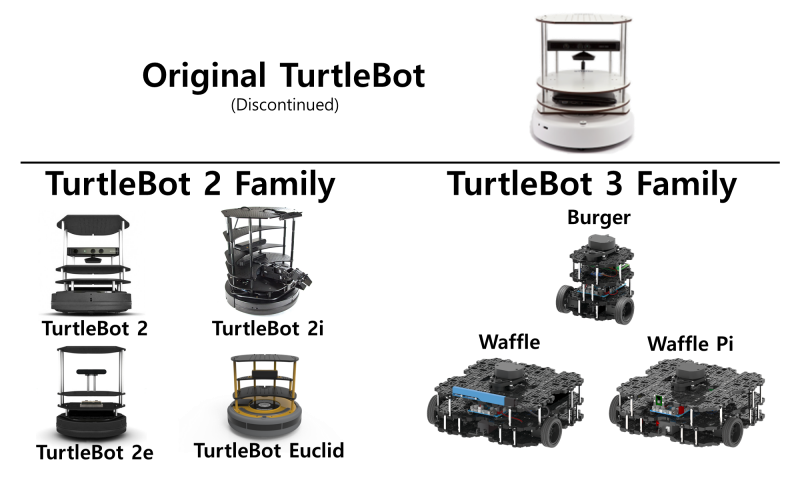
\includegraphics[scale=.5]{turtlebot_family.png}

\begin{enumerate}
	\item Update your linux system before you get started. 
	\begin{minted}{text} 
	sudo apt update
	\end{minted}

	\item Install the necessary nodes into your ROS system. This tutorial comes from \href{http://emanual.robotis.com/docs/en/platform/turtlebot3/simulation/#simulation} {here.} 
    	
    	{\bf turtlebot3 }
	\begin{minted}{text} 
	sudo apt install ros-|\rosdistro|-turtlebot3
	\end{minted}
 	 {\bf turtlebot3\_simulations}
	\begin{minted}{text} 
	sudo apt install ros-|\rosdistro|-turtlebot3-simulations
	\end{minted}
 	{\bf turtlebot3\_gazebo}
	\begin{minted}{text} 
	sudo apt install ros-|\rosdistro|-turtlebot3-gazebo
	\end{minted}


%    \item Next install the physical 'turtlebot' drivers into your ROS system. This step is only necessary if you are using a real turtlebot. \href{http://wiki.ros.org/Robots/TurtleBot} {Link Here} 
%   \begin{minted}{text}  
%(sudo apt install ros-|\rosdistro|-turtlebot ros-|\rosdistro|-turtlebot-apps
%ros-|\rosdistro|-turtlebot-interactions ros-|\rosdistro|-turtlebot-simulator 
%ros-|\rosdistro|-kobuki-ftdi ros-|\rosdistro|-rocon-remocon 
%ros-|\rosdistro|-rocon-qt-library ros-|\rosdistro|-ar-track-alvar-msgs})
%\end{minted}
%    
\newpage
    \item Test the simulator. First set the environment variable TURTLEBOT\_MODEL. Add this line to the .bashrc script so you do not have to do it for each terminal. \\
	\begin{minted}{text} 
	export TURTLEBOT3_MODEL=burger
	\end{minted}
	Then turn on the simulator. 
	\begin{minted}{text} 
	roslaunch turtlebot3_gazebo turtlebot3_world.launch
	\end{minted}

	You should see the gazebo window open containing your robot. Test that the keyboard drives the robot. This may take some time.
	\begin{minted}{text} 
	roslaunch turtlebot3_teleop turtlebot3_teleop_key.launch
	\end{minted}
	    
	    \item Now turn on the node to produce robot data in the simulated world.  \\

	\begin{minted}{text} 
	roslaunch turtlebot3_gazebo turtlebot3_simulation.launch
	\end{minted}

	Open RVIZ to view the data. This is a very useful tool. 	
	\begin{minted}{text} 
	roslaunch turtlebot3_gazebo turtlebot3_gazebo_rviz.launch
	\end{minted}
	
	\item Next we are going to learn about SLAM and GMAPPING ! Please see the tutorial referenced above if you are ready to proceed.\\
%    \begin{itemize}
%    
%        \item {\fontfamily{qcr}\selectfont  \hspace{5mm} \pthname maze.png}
%        \item {\fontfamily{qcr}\selectfont  \hspace{5mm} \pthname maze.yaml}
%        \item {\fontfamily{qcr}\selectfont  \hspace{5mm} \pthname stage/maze.world}
%    
%    \end{itemize}

%    \item First try the simulator in the demo world called {\it maze}. We will export the files as {\it environment variables}
%
%    {\fontfamily{qcr}\selectfont  \hspace{5mm} \$ export TURTLEBOT\_STAGE\_MAP\_FILE=\\"\pthname maze.yaml"}\\
% 
%    {\fontfamily{qcr}\selectfont  \hspace{5mm} \$ export TURTLEBOT\_STAGE\_WORLD\_FILE=\\"\pthname stage/maze.world"}\\
%    
%    \item Now use the launch file (available upon install) to start the simulator.\\
%    {\fontfamily{qcr}\selectfont  \hspace{5mm} \$ roslaunch turtlebot\_stage turtlebot\_in\_stage.launch}
%    
%    \item Now you can modify the world you have just simulated. To do this copy all three files and rename them something sensible. Open the {\it .png} file with any image editor, and draw on it and save. You also need to modify just a few lines in the {\it .yaml} file and the {\it .world} file. (Note: This step will be detailed in the next tutorial. Continue at your own risk or contact me for help.)
%    
%     \item Did you notice an error when you turned the node on? We can fix that.  \\\\
%    
%    	 {\fontfamily{qcr}\selectfont  \hspace{5mm} \$ sudo  gedit /opt/ros/\rosdistro/share/gmapping/nodelet\_plugins.xml}\\\\
%    	 
%    	 Copy the code below into the new file. This a bug related to moving to `kinetic'.\\
%    \lstset{language=XML}
%     \begin{lstlisting}
%
%<library path="lib/libslam_gmapping_nodelet">
%    <class name="SlamGMappingNodelet" type="SlamGMappingNodelet" base_class_type="nodelet::Nodelet">
%        <description>
%            Nodelet ROS wrapper for OpenSlams Gmapping.
%        </description>
%    </class>
%</library>
%      \end{lstlisting}
%
%\vspace{5mm}    Now run your node again.
\end{enumerate}
\end{document}

